% Overleaf-ready provisional XP 2027 manuscript.
% Uses Springer's official Computer Science Proceedings class (v2.25, 2026-09-03).
% Reconfirm the XP 2027 track, page limit, review model, and template when the call appears.
% Before submission, confirm both authors' email addresses, ORCID IDs, and final approval.
\documentclass[runningheads]{llncs}

\usepackage[T1]{fontenc}
\usepackage{newtxtext}
\usepackage[varvw]{newtxmath}
\usepackage{graphicx}
\usepackage{xcolor}
\usepackage{tikz}
\usetikzlibrary{arrows.meta,positioning}
\usepackage{hyperref}
\renewcommand\UrlFont{\color{blue}\rmfamily}
\urlstyle{rm}
\emergencystretch=3em
\hypersetup{
  pdftitle={Can Organizational History Inform What Agile Teams Improve Next? A Walk-Forward Study of 87 Teams},
  pdfauthor={Erez Morabia; Shmuel Tyszberowicz},
  pdfsubject={Provisional XP 2027 research paper}
}

\definecolor{xpblue}{HTML}{2455A4}
\definecolor{xpbluegray}{HTML}{65758B}
\definecolor{xpteal}{HTML}{16827A}
\definecolor{xplight}{HTML}{EEF3F8}

\begin{document}

\title{Can Organizational History Inform What Agile Teams Improve Next?}
\subtitle{A Walk-Forward Study of 87 Teams}
\titlerunning{Can Organizational History Inform What Agile Teams Improve Next?}

\author{Erez Morabia\inst{1} \and Shmuel Tyszberowicz\inst{1}}
\authorrunning{E. Morabia and S. Tyszberowicz}
\institute{The Open University of Israel, Ra'anana, Israel}

\maketitle

\begin{abstract}
Agile maturity assessments record how teams change over time, but organizations rarely test whether this history can inform what a team considers next. We study whether longitudinal assessments can rank two practices associated with a team's next recorded improvements, and whether peer similarity and practice transitions add value beyond time-aware organizational popularity. The retrospective dataset contains 654 unique team-month observations from 87 teams, 30 retained practices, and ten organization-wide snapshots between January and November 2020. A global policy is selected for each prediction month using only earlier outcomes whose windows have closed. The prespecified primary cohort contains 121 outcome-bearing cases from 42 teams over five prediction months. The selected blend obtained 58.0\% monthly macro Conditional Hit Rate@2 (95\% team-cluster bootstrap interval 47.1\%--68.2\%), versus 30.6\% for an exact candidate-aware random expectation. However, independently selected time-aware popularity obtained 55.7\%; the paired gap was only 2.3 percentage points (0.0--5.2), and the arms were identical in three of five months. A stricter team-complete sensitivity removed one case and yielded 57.3\% versus 54.9\%. Thus, organizational history contains ranking signal, although most of it is recovered by a simple frequency baseline and the study does not establish incremental value from peer and transition signals. An exploratory analysis of all 298 complete-window recommendable cases yielded 23.1\% observed alignment for the blend and 22.2\% for popularity. We contribute a reusable baseline-first protocol that separates historical signal from incremental personalization. For human-centered AI decision support, longitudinal data can provide hypotheses for coach-team deliberation, while added signals require stable, decision-relevant gains under prediction-time evaluation.

\keywords{Agile software development \and Artificial intelligence \and Maturity assessment \and Recommender systems \and Temporal validation \and Decision support}
\end{abstract}

\section{Introduction}

Agile assessments can expose many practices below a target maturity level without resolving a recurring coaching decision: what should this team consider next? Such decisions often draw on local judgment or static roadmaps, while longitudinal organizational histories offer another source of evidence. An adaptive recommender could combine experience from similar teams, typical practice sequences, and recent organizational movement. In an era of AI-assisted software work, the first question is whether these histories contain useful ranking signal; the second is whether personalization adds information beyond an inspectable organization-wide frequency rule.

We formulate next-practice guidance as top-two ranking over practices not already at maximum maturity. The intended output is a hypothesis for coach-team deliberation, not an automated prescription. An observed maturity-score increase is treated as the event to rank; it is not assumed to represent a durable capability change or an effect caused by a recommendation.

The study asks:
\begin{itemize}
\item \textbf{RQ1:} How effectively can organization-specific maturity histories identify practices associated with a team's next recorded improvement under walk-forward evaluation?
\item \textbf{RQ2:} What incremental value and stability do peer similarity and practice-transition evidence provide beyond time-aware organizational popularity?
\end{itemize}

We contribute: (1) evidence that organization-specific maturity histories can inform next-practice ranking; (2) a transparent three-signal method; and (3) a reusable baseline-first protocol that keeps feature evidence, candidate construction, outcome closure, and policy selection on their correct sides of prediction time. Comparison with random ranking tests whether organizational history contains signal, while time-aware popularity isolates the incremental value of peer and transition evidence. Here the first condition holds and the second is not established.

\section{Background and Related Work}

\subsection{Agile Improvement and Maturity}

Agile research emphasizes contextual evidence rather than universal transformation recipes~\cite{dyba2008empirical,dikert2016large}. Maturity models can structure reflection, but reviews find limited validation of agile maturity models and low-strength evidence on combining agile development with CMMI~\cite{henriques2017maturity,silva2015cmmi}. We therefore use maturity scores as longitudinal organizational observations, not validated measures of delivery performance.

\subsection{AI Support for Agile Work}

A systematic review finds that intelligent techniques in agile software development primarily support decisions, while empirical evaluation remains limited~\cite{perkusich2020intelligent}. More recent practitioner research prioritizes context-aware support for requirements, communication, and Scrum processes~\cite{fujs2026scrumai}. XP studies examine AI's role in teamwork~\cite{kwok2026aiteamwork}, customized meeting assistants~\cite{cabrero2024assistants}, and practitioners' expectations about human-AI collaboration~\cite{planotscher2026collaboration}. These studies also reinforce a socio-technical boundary: AI may inform planning and reflection, but people remain accountable for context, trust, feasibility, and value.

Our method is not a generative-AI system. It is a transparent statistical recommender situated within this broader class of AI-enabled decision support. Its relevance lies in testing whether historical patterns can support process guidance and how much additional information personalization contributes before such guidance is presented to teams.

\subsection{Recommendation and Evaluation}

Recommendation systems for software engineering have supported artifacts, experts, tools, and engineering decisions~\cite{gasparic2016recommend}. Process-model recommendation shows that project attributes can inform method selection~\cite{song2016process}. Related work guides agile improvement through a goal-oriented maturity map~\cite{packlick2007maturity}, constructs assessment-based software-process recommendations~\cite{choi2012remo}, and recommends improvement actions from individual developer performance~\cite{raza2017webprocesspair}. These targets differ from ranking the next observed practice change in longitudinal team assessments.

Evaluation choices can dominate recommender results. Reproducibility work calls for explicit data splits, candidate sets, and implementation details~\cite{bellogin2021accountability}. Popularity is both a competitive strategy and a possible source of narrowing or reinforcement, so it requires application-specific interpretation~\cite{klimashevskaia2024popularity}. Offline metrics must match the intended ranking task~\cite{herlocker2004evaluation}, and temporal splits should predict later interactions from past evidence without training on future information~\cite{bellogin2021accountability}. These concerns motivate our walk-forward design and the treatment of popularity as the principal comparator rather than a token baseline.

An earlier public, unpublished MSc project report describes the prototype and headline backtest~\cite{morabia2026project}. This paper extends that work with team-cluster uncertainty, fixed ablations, a frozen protocol, current literature positioning, and a conference-focused research argument.

On 13 September 2026, a structured scoping search screened the first 20 Crossref records for each of four query families: ``agile practice'' recommender, ``agile maturity'' recommendation, ``software process'' recommendation method, and ``agile transformation'' sequence mining. OpenAlex abstract and availability records supported shortlisting. Records were included when they addressed agile maturity/improvement or software-process recommendation or selection; general transformation commentary, non-software recommenders, and artifact/API recommendation were excluded. Table~\ref{tab:gap} compares the four closest studies. NR means that a feature was not reported in the screened title or abstract, not that the full text proves its absence. This scoping check sharpens but does not exhaustively establish the novelty claim.

\begin{table}[t]
\caption{Closest screened studies. NR means not reported in the screened title or abstract.}
\label{tab:gap}
\centering
\scriptsize
\setlength{\tabcolsep}{2.5pt}
\begin{tabular}{@{}p{1.45cm}p{2.75cm}p{1.65cm}p{1.65cm}p{1.55cm}@{}}
\hline
\textbf{Study} & \textbf{Guidance target} & \textbf{Longitudinal teams} & \textbf{Next observed practice} & \textbf{Walk-forward baseline} \\
\hline
Packlick~\cite{packlick2007maturity} & Agile maturity-guided change & NR & NR & NR \\
Choi et al.~\cite{choi2012remo} & Process-improvement actions & NR & NR & NR \\
Raza et al.~\cite{raza2017webprocesspair} & Developer-improvement actions & NR & NR & NR \\
Song et al.~\cite{song2016process} & Software-process model & NR & No & NR \\
This study & Team practice top two & Yes & Yes & Yes \\
\hline
\end{tabular}
\end{table}

\section{Study Design}

\subsection{Setting and Observations}

The source is a repeated maturity assessment from one multinational telecommunications organization. It contains 655 rows and 654 unique team-month observations after deterministically retaining the final occurrence of one duplicate. There are 87 teams and ten dated organization-wide snapshots from 7 January to 4 November 2020. Thirty-five practice columns use a 0--3 scale; practices with more than 90\% missing values are excluded, leaving 30, and retained scores are normalized to 0--1. Three teams have only one observation. Team identities are used only to retain longitudinal clusters and never appear in the evidence package.

The sanitized XP submission package does not contain team aliases, row-level observations, or source workbooks. It contains analysis code, aggregate results, deterministic tests, and a schema-compatible synthetic example; organizational data are excluded from its Apache-2.0 license. The broader public repository associated with the prior MSc project~\cite{morabia2026project} remains separate and tracks the source workbooks and practice documentation under the reported verbal authorization described in the disclosures. That separation limits independent reproduction from the conference artifact and does not make the broader repository non-identifying or grant a data license.

\subsection{Prediction Cases and Estimand}

For prediction month $m$, the baseline is a team's latest recorded snapshot strictly before $m$. A case is recommendable when a baseline exists and at least two practices are below maximum. The eligible candidate set is fixed before scoring. The outcome is the union of eligible practices whose score increases within up to the next three recorded team snapshots. A case enters the primary ranking cohort only when this set is nonempty.

The prespecified primary scope uses five prediction months whose three-snapshot horizon is globally observable. It contains 121 outcome-bearing cases from 42 of the 87 teams. The estimand is therefore conditional ranking alignment: if an eligible practice later increases, does either recommendation identify one? It does not estimate whether a team will improve or whether advice causes change.

A stricter audit found 298 recommendable cases with exactly three subsequent team snapshots. Of these, 120 (40.3\%) had an eligible increase and 178 (59.7\%) did not. The strict outcome-bearing sensitivity therefore contains 120 cases from 41 teams; it was added after protocol freeze and cannot replace the primary result based on favorability. A separate post-protocol analysis retains all 298 cases, assigns zero observed alignment when no eligible increase occurred, and estimates retrospective alignment across recommendable cases rather than conditional ranking performance.

\subsection{Temporal Boundary}

All features are evaluated at the target baseline. Peer outcomes are capped at that baseline; practice transitions and popularity use only earlier organizational changes. A previous prediction month can tune a policy only after its full outcome window closes before the target month. The same precomputed cohort is scored by every method (Fig.~\ref{fig:boundary}).

\begin{figure}[t]
\centering
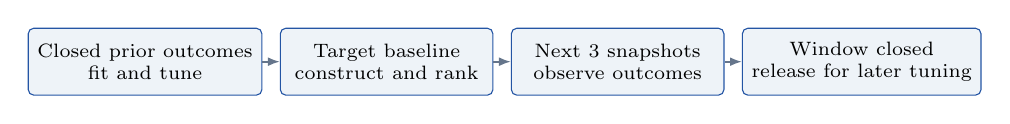
\begin{tikzpicture}[
  node distance=2.2mm,
  every node/.style={font=\scriptsize, align=center},
  box/.style={draw=xpblue, rounded corners=2pt, fill=xplight, minimum width=2.7cm, minimum height=0.85cm},
  arr/.style={-{Latex[length=1.5mm]}, semithick, draw=xpbluegray}
]
\node[box] (closed) {Closed prior outcomes\\fit and tune};
\node[box, right=of closed] (baseline) {Target baseline\\construct and rank};
\node[box, right=of baseline] (future) {Next 3 snapshots\\observe outcomes};
\node[box, right=of future] (release) {Window closed\\release for later tuning};
\draw[arr] (closed) -- (baseline);
\draw[arr] (baseline) -- (future);
\draw[arr] (future) -- (release);
\end{tikzpicture}
\caption{Prediction-time boundary. A prior month can tune a later policy only after its outcome window closes.}
\label{fig:boundary}
\end{figure}

\section{Recommendation and Policy Selection}

\subsection{Evidence Signals}

\textbf{Peer similarity.} Cosine similarity compares the target baseline with historical snapshots from other teams. For a candidate practice, an eligible peer contributes its similarity multiplied by the peer's largest increase during its next two snapshots, provided neither snapshot occurs after the target baseline. Duplicate peers are removed before the top $k$ are retained.

\textbf{Practice transitions.} Directed transitions are learned from consecutive improvement-bearing steps. Practices that increased in the target team's two preceding snapshots trigger empirical probabilities for typical successors. Simultaneous increases do not create directed edges.

\textbf{Popularity.} Historical popularity counts all practice increases observed before the baseline. Recent popularity uses only the organizational transition immediately preceding the baseline. A recency parameter mixes the two.

For candidate $p$, the final score is
\begin{equation}
\mathrm{score}(p)=w_sS(p)+w_tT(p)+w_pP(p), \qquad
P(p)=rP_{\mathrm{recent}}(p)+(1-r)P_{\mathrm{historical}}(p),
\end{equation}
where nonnegative weights sum to one. Components are normalized in their documented scopes. The two highest candidates are returned, using practice name as the final deterministic tie-break.

\subsection{Walk-Forward Selection and Comparators}

The policy grid contains 675 combinations: peer count in $\{5,10,19\}$; minimum similarity in $\{0,0.5,0.75\}$; 15 three-factor weight triples on a 0.25 grid; and recency in $\{0,0.25,0.5,0.75,1\}$. One global policy is selected each month by mean Hit Rate@2 on completed prior months. Before any outcome window has closed, a fixed policy uses popularity alone with $r=0.5$.

The strongest comparator independently selects among five pure-popularity policies using the same temporal rule. An exact candidate-aware random expectation controls for the number of eligible and improved practices. Eight fixed, untuned ablations isolate historical popularity, recent popularity, similarity, transitions, the equal three-factor blend, and the three equal-weight signal pairs.

\section{Evaluation}

Hit Rate@2 is one when either recommendation is in the actual-positive set. Cases are averaged within prediction month, then the five month-level values receive equal weight. Supporting metrics are Precision@2, Recall@2, mean reciprocal rank (MRR), practice coverage, and pooled descriptive Hit Rate@2.

For candidate count $n$, improved-candidate count $k$, and recommendation depth $d=\min(2,n)$, exact random Hit Rate is $1-\binom{n-k}{d}/\binom{n}{d}$. This case-level expectation is aggregated identically to the observed methods.

Uncertainty uses 10,000 paired team-cluster bootstrap replicates with seed 22997~\cite{efron1979bootstrap,deen2020clusterbootstrap}. A replicate samples team identities with replacement, retains all selected cases for each sampled team, and recomputes monthly macro means. These percentile intervals are conditional on the monthly policies fitted to the observed histories: policy selection is not repeated inside each replicate. They describe within-organization team-sampling instability, not uncertainty from having only five months, model selection, measurement error, or transport to another company.

A post-protocol robustness bootstrap repeats the full walk-forward policy choice within each team-cluster replicate, using the unchanged 675-policy grid and the same outcome-closure boundary. It therefore incorporates variability in which blend and popularity policies are selected. Months without a completed prior window retain the fixed bootstrap policy. This analysis uses 10,000 replicates with seed 22999 and is reported separately from the prespecified intervals.

The research questions, primary scope, metrics, comparators, and fixed ablations were frozen before the extended evidence build. Automated tests pin cohort counts, temporal boundaries, deterministic bootstrap output, and the absence of team identifiers from aggregate evidence. The all-recommendable analysis was added after protocol freeze and is explicitly exploratory; it cannot replace the primary estimand.

\section{Results}

The selected blend reached 58.0\% monthly macro Conditional Hit Rate@2 (47.1\%--68.2\%) and 58.7\% pooled Hit Rate@2. Time-aware popularity reached 55.7\% (45.2\%--65.6\%). Their paired gap was 2.3 points (0.0--5.2). The arms were identical in the first three months because neither had a completed prior window; the only differentiated months favored the blend by 4.2 and 7.4 points. Thus the data establish organizational ranking signal but not a reliable incremental advantage from the peer and transition components.

\begin{figure}[t]
\centering
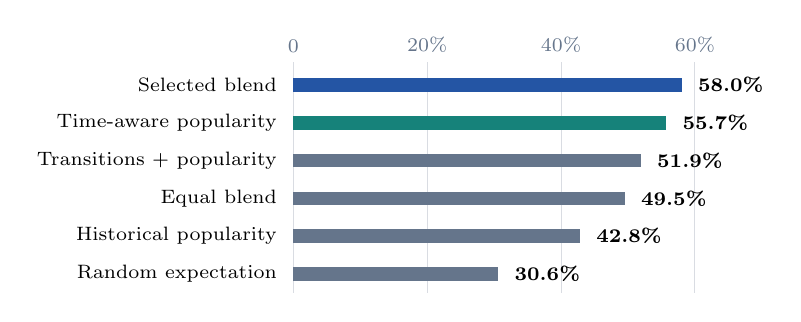
\begin{tikzpicture}[x=0.085cm,y=0.48cm,font=\scriptsize]
\draw[xpbluegray!35] (0,-0.5) -- (0,5.6);
\foreach \x/\lab in {0/0,20/20\%,40/40\%,60/60\%} {
  \draw[xpbluegray!25] (\x,-0.5) -- (\x,5.6);
  \node[above,xpbluegray] at (\x,5.6) {\lab};
}
\foreach \name/\value/\y/\barcolor in {
  {Selected blend}/58.0/5/xpblue,
  {Time-aware popularity}/55.7/4/xpteal,
  {Transitions + popularity}/51.9/3/xpbluegray,
  {Equal blend}/49.5/2/xpbluegray,
  {Historical popularity}/42.8/1/xpbluegray,
  {Random expectation}/30.6/0/xpbluegray} {
  \node[anchor=east] at (-1,\y) {\name};
  \fill[fill=\barcolor] (0,\y-0.18) rectangle (\value,\y+0.18);
  \node[anchor=west,font=\scriptsize\bfseries] at (\value+1,\y) {\value\%};
}
\end{tikzpicture}
\caption{Primary monthly macro Conditional Hit Rate@2. Popularity is a substantive comparator.}
\label{fig:results}
\end{figure}

\begin{table}[t]
\caption{Primary per-month Conditional Hit Rate@2.}
\label{tab:monthly}
\centering
\small
\begin{tabular}{@{}lrrrr@{}}
\hline
\textbf{Prediction month} & \textbf{Cases} & \textbf{Blend} & \textbf{Popularity} & \textbf{Difference} \\
\hline
2020-05 & 21 & 28.6\% & 28.6\% & +0.0 \\
2020-06 & 22 & 63.6\% & 63.6\% & +0.0 \\
2020-07 & 27 & 66.7\% & 66.7\% & +0.0 \\
2020-08 & 24 & 79.2\% & 75.0\% & +4.2 \\
2020-09 & 27 & 51.9\% & 44.4\% & +7.4 \\
\hline
Monthly macro & 121 & 58.0\% & 55.7\% & +2.3 pp \\
\hline
\end{tabular}
\end{table}

The exact random expectation was 30.6\% (25.0\%--36.7\%), producing a paired blend gap of 27.4 points (17.5--36.5). Supporting blend results were Precision@2 35.6\%, Recall@2 17.6\%, MRR 45.9\%, and practice coverage 53.3\%.

All fixed ablations are reported. Transitions plus popularity was strongest at 51.9\%, followed by the equal blend at 49.5\%, similarity plus transitions at 45.3\%, similarity plus popularity at 45.1\%, historical popularity at 42.8\%, similarity alone at 42.4\%, recent popularity at 40.1\%, and transitions alone at 15.7\%. Several paired intervals against the selected blend include zero; ablations are descriptive rather than proof of component effects.

The 120-case strict team-complete sensitivity yielded 57.3\% for the blend, 54.9\% for time-aware popularity, and 30.3\% for random expectation. The all-month sensitivity, which includes two right-censored prediction months, contained 151 cases over seven months and yielded 50.9\%, 47.5\%, and 28.0\%, respectively. Neither sensitivity changes the conclusion.

Across all 298 complete-window recommendable cases, including 178 without an eligible recorded increase, exploratory monthly macro observed alignment was 23.1\% for the blend (16.1\%--30.4\%), 22.2\% for time-aware popularity (15.4\%--29.4\%), and 12.2\% for random expectation (8.8\%--16.0\%). The paired blend-popularity gap was 0.9 points (0.0--2.2). This is not an improvement-occurrence forecast: a zero can mean either that no eligible practice increased or that an observed increase was not ranked in the top two.

When policy selection was repeated inside each bootstrap replicate, the blend interval was 44.6\%--65.7\%, popularity was 40.7\%--64.8\%, and the paired gap widened to -4.4 to 12.5 points. In the two adaptive primary months, resampling selected 15 and 31 distinct blend policies; the observed-data policies were modal but appeared in only 32.6\% and 21.0\% of replicates. Thus, limited prior outcome windows make the selected configuration unstable, reinforcing rather than weakening the conclusion that incremental personalization is unestablished.

\section{Discussion and Threats to Validity}

The study answers RQ1 positively but narrowly: past organizational behavior contains signal for ranking later recorded practice increases and can provide hypotheses for coach-team deliberation. RQ2 receives a mostly negative answer. Similarity and transition signals did not demonstrate stable incremental value beyond a carefully selected popularity strategy. With only two differentiated months, the 2.3-point gain does not establish their added decision value.

This result matters for AI-era agile tooling. A system can appear personalized while mainly reproducing common organizational behavior. Popularity should therefore be displayed as an explicit comparator and possible explanation, not hidden inside a blended score. Coaches and teams should see the source of each suggestion and retain authority over whether it is feasible or valuable. A prospective study should measure perceived explanation quality, decision changes, practice adoption, and delivery outcomes, including potential reinforcement of already popular practices.

\subsection{A Baseline-First Evaluation and Use Gate}

The protocol supports a four-question gate for an organization considering data-informed agile guidance: (G1) were all features, candidates, tuning outcomes, and comparators available at prediction time; (G2) does personalization improve on an independently tuned, time-aware simple baseline by a practically meaningful margin; (G3) is that gain stable across prediction periods and sensitivity scopes; and (G4) can users inspect the baseline, added signal sources, and uncertainty while retaining decision authority? Failing G1 invalidates the evaluation. Failing G2 or G3 means the personalized components should not be presented as superior; organizational history may still provide useful baseline evidence while more data are collected. G4 is required before prospective use, irrespective of offline accuracy.

Applied here, G1 is satisfied by construction, but G2 and G3 are not: the paired gain is 2.3 points with an interval touching zero, and the methods differ in only two primary months. G4 is a design requirement rather than an evaluated outcome. The evidence therefore supports continued baseline monitoring and a prospective human-centered evaluation, not deployment of the blend as a proven improvement.

\subsubsection{Construct validity.} Score increases may reflect rater changes, measurement noise, or reassessment rather than durable capability. Although practice documentation is available in the prior-project repository, the instrument's measurement validity has not been independently established. A three-snapshot union ranks near-term change, not necessarily the single next action.

\subsubsection{Internal and conclusion validity.} Unobserved organizational initiatives may drive both popularity and team changes. The 675-policy search operates on at most two completed training months for the differentiated primary predictions. The prespecified bootstrap does not refit that selection, while the post-protocol refit analysis shows substantial policy instability and a paired interval spanning zero. Five primary months provide little temporal variation.

\subsubsection{Selection and use validity.} The conditional cohort excludes 178 of 298 complete-window recommendable cases with no recorded increase. Consequently, 58.0\% must not be read as an unconditional success probability. Retrospective alignment cannot show that presenting a recommendation would cause adoption or better outcomes. The exploratory 23.1\% result restores those cases but conflates absence of an eligible increase with ranking misses, so it is observed alignment, not a calibrated probability that a recommendation will succeed.

\subsubsection{External and reproducibility validity.} One organization, one 2020 assessment vocabulary, and 42 primary-cohort teams limit transportability. Code and aggregate evidence are reproducible from the sanitized artifact, but the XP package alone cannot independently reproduce the empirical results. The separate public prior-project repository contains the source workbooks but carries no organizational-data license. The submission relies on the reported verbal approval described below and on a stricter aggregate-only XP release policy.

\section{Conclusion}

The three-signal recommender aligned one of two suggestions with a later recorded increase in 58.0\% of conditional cases and substantially exceeded random expectation. This supports the use of longitudinal organizational history as a source of hypotheses about what teams may improve next, not as proof that recommendations cause adoption or outperform human judgment. Time-aware popularity achieved 55.7\%, and the richer approach was meaningfully different in only two months, so incremental value from peer and transition evidence remains unestablished. The defensible contribution is an auditable temporal evaluation for data-informed agile practice guidance whose evidence and limits remain visible to the people making the decision.

\section*{Data Availability and Disclosures}

The organizational dataset is excluded from the sanitized XP package. No formal ethics approval was required for this retrospective analysis; XP materials contain aggregate results, use an unnamed organizational description, and omit team identifiers. The first author created and maintained the workbooks and reports that the responsible manager verbally approved for academic use and knew would be public in the prior-project GitHub repository; no written record exists. That repository is not the conference artifact, does not guarantee non-inferability of the organization, and grants no license to the organizational data. This research received no external funding. The first author was formerly employed by the source organization and participated in data collection in that professional role; the employment ended more than five years ago, and the project was developed years later. Software and original documentation are Apache-2.0 licensed; organizational data are excluded. The unpublished public MSc report~\cite{morabia2026project} is prior work. Generative AI assistance used for planning, language refinement, and methodological checks will be disclosed under the final venue rule; the authors verified and remain accountable for the work.

\begin{credits}
\subsubsection{Author Contributions}
E.M. contributed conceptualization, methodology, software, validation, formal analysis, investigation, data curation, visualization, and writing--original draft. S.T. contributed supervision, methodological guidance, and writing--review and editing. Both authors reviewed the manuscript and will approve the final version before submission.

\subsubsection{Funding}
This research received no external funding.

\subsubsection{\discintname}
The authors have no competing interests to declare that are relevant to the content of this article.
\end{credits}

\bibliographystyle{splncs04}
\bibliography{references}

\end{document}
